\chapter{Experimental results and conclusions}
\section{Results}
Our propose in a nutshell is a new substitutive method of Watershed transform. The following results are obtained using an Acer Aspire E1 laptop with 8 gb of RAM. the figure \ref{fig:alltheprocess} show all the process starting from the gray scale image to the mask used to find only the leukocytes.
\begin{figure}[htbp]
    \centering
    \begin{subfigure}[b]{0.45\textwidth}
        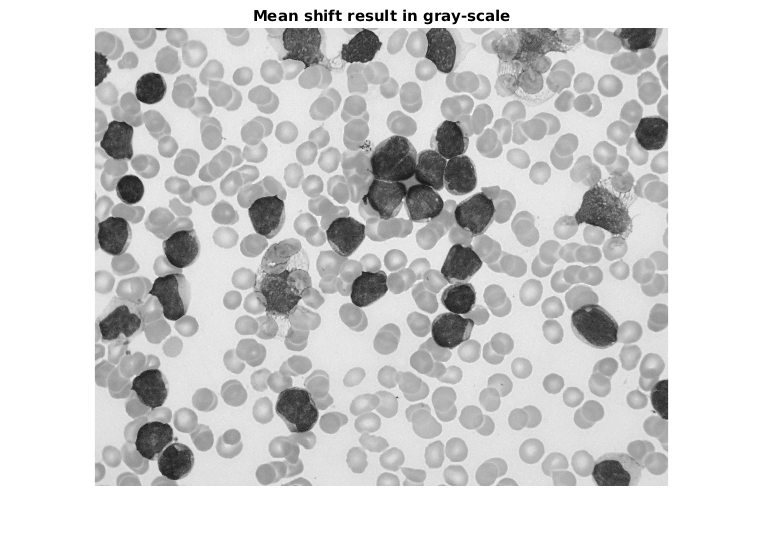
\includegraphics[width=\textwidth]{img/final/figure1.png}
        \caption{ }
        \label{fig:fig1}
    \end{subfigure}
      %(or a blank line to force the subfigure onto a new line)
    \begin{subfigure}[b]{0.45\textwidth}
        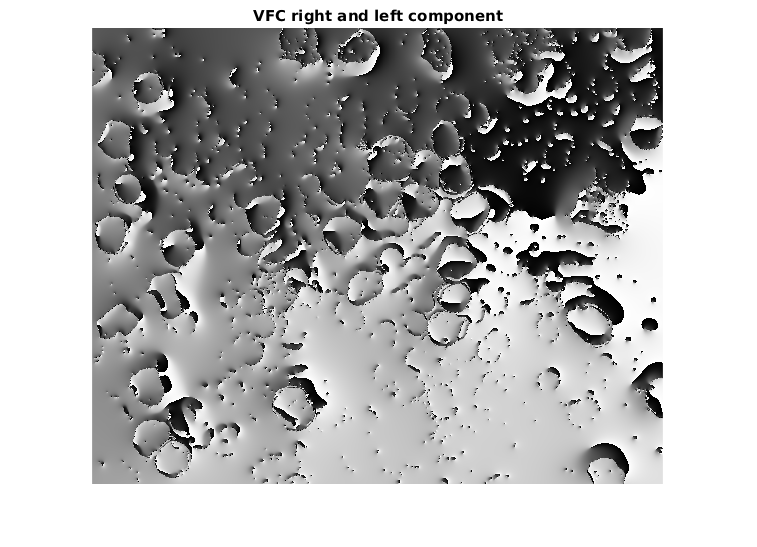
\includegraphics[width=\textwidth]{img/final/figure2.png}
        \caption{ }
        \label{fig:fig}
    \end{subfigure}
    \begin{subfigure}[b]{0.45\textwidth}
        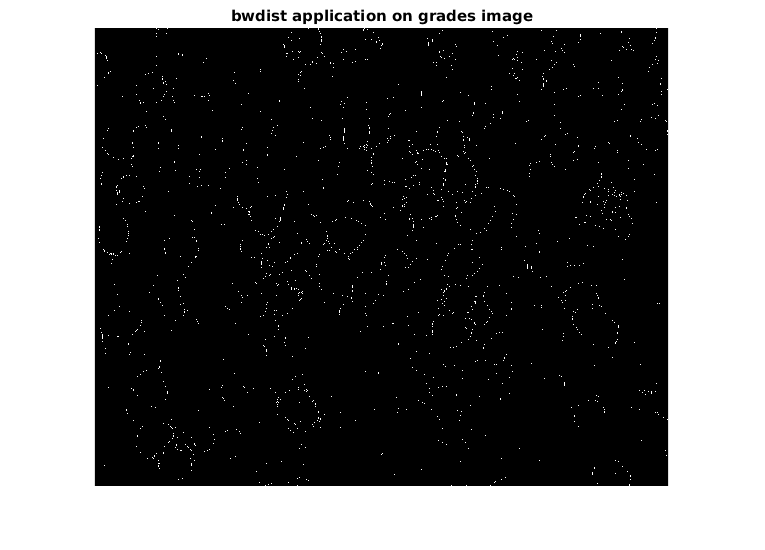
\includegraphics[width=\textwidth]{img/final/figure3.png}
        \caption{ }
        \label{fig:fig3}
    \end{subfigure}
    \begin{subfigure}[b]{0.45\textwidth}
        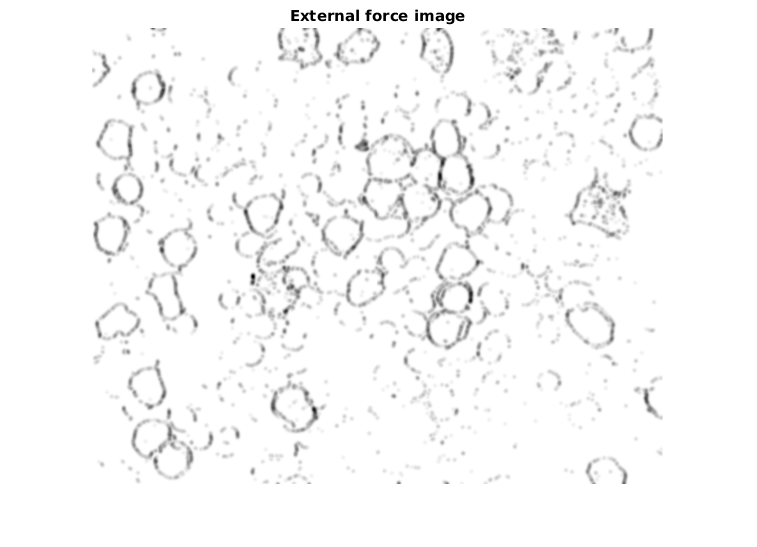
\includegraphics[width=\textwidth]{img/final/figure4.png}
        \caption{ }
        \label{fig:fig4}
    \end{subfigure}
    \begin{subfigure}[b]{0.45\textwidth}
        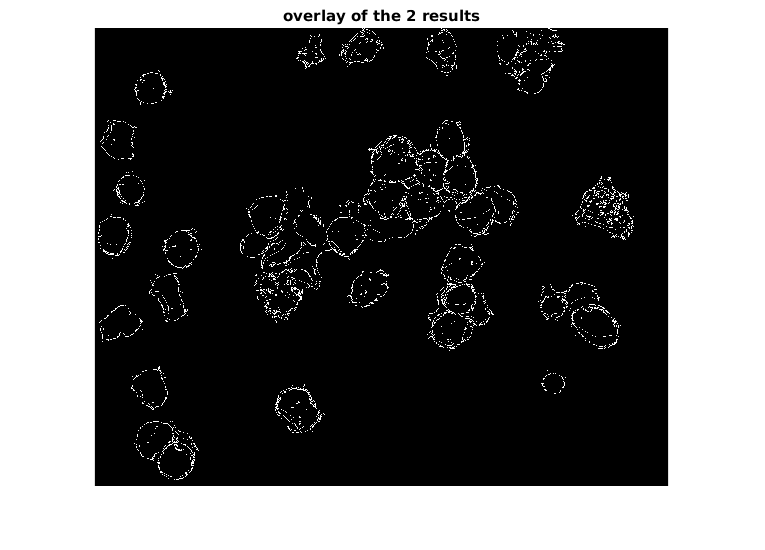
\includegraphics[width=\textwidth]{img/final/figure5.png}
        \caption{ }
        \label{fig:fig5}
    \end{subfigure}
    \begin{subfigure}[b]{0.45\textwidth}
        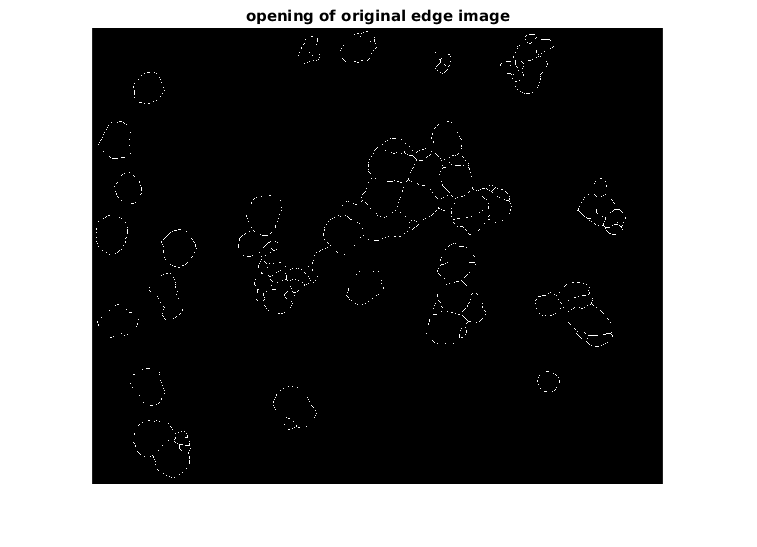
\includegraphics[width=\textwidth]{img/final/figure6.png}
        \caption{ }
        \label{fig:fig6}
    \end{subfigure}
    \begin{subfigure}[b]{0.45\textwidth}
        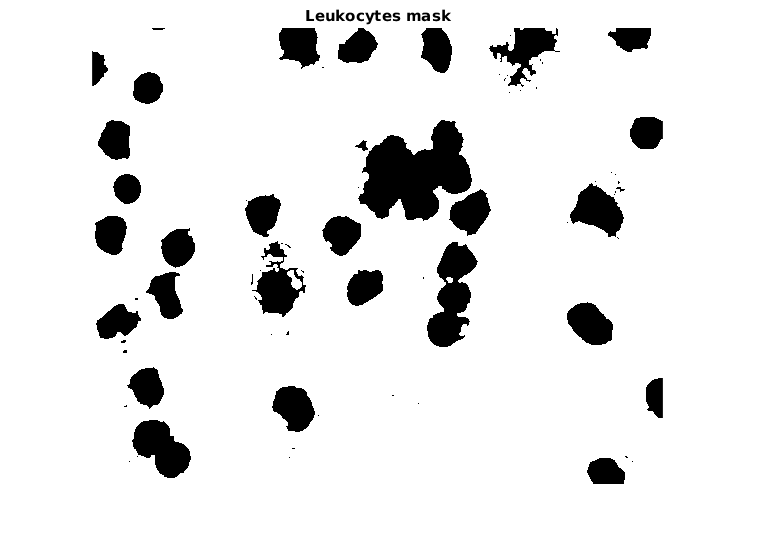
\includegraphics[width=\textwidth]{img/final/figure7.png}
        \caption{ }
        \label{fig:fig7}
    \end{subfigure}

    
    \caption{(a) Mean shift result in gray scale,(b) VFC u and v components,(c) Distance transform on grades image, (d) External force image, (e) overlay of two results, (f) Opening of initial edge image, (g) Leukocytes mask}
    \label{fig:alltheprocess}
\end{figure}
The last two figures \ref{fig:fig8} \ref{fig:fig9} show the real result of the segmentation

\begin{figure}
\centering
	\begin{center}
		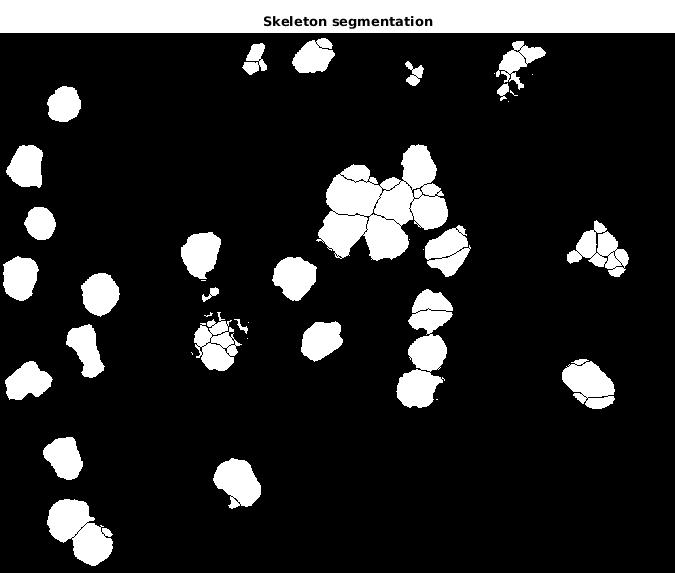
\includegraphics[scale=0.5]{img/final/figure8.png}
		\caption{skeleton segmentation}
		\label{fig:fig8}
	\end{center}
\end{figure}
\begin{figure}
\centering
	\begin{center}
		
\includegraphics[scale=0.5]{img/final/figure9.png}
		\caption{Removing of little area to count the number of leukocytes}
		\label{fig:fig9}
	\end{center}
\end{figure}
\bigskip

As it possible to see, between the two images there are some differences. the first one is, removing the small areas by the image we are going to lose the element on the right of the image. This is happened because it was artefact caused by the Giemsa stain method, then is obvious that it's not well segmented because under the stain is not present  leukocyte. The result of the counting in this case is 29. The algorithm fails the result because two leukocytes have a visualization problem and inside the nuclei have a line that divide in tow sides the cells.
Working with cropped images we obtain a better result because we have to analyse less cells and as a consequence we have an increase of the speed as is explained in the table \ref{statistics}.
\begin{table}
\centering
\begin{tabular}{|c|c|c|c|}
\hline 
name & cropped & time & Number of recognized cells / number of real cells\\ 
\hline 
image 5 & no & 45.050214 & 29/27\\ 
\hline 
image 5 & yes & 2.214306 & 7/7\\ 
\hline 
image 13 & no & 31.827737 & 11/11 \\ 
\hline 
image 13 & yes & 1.189616 & 4/4 \\ 
\hline 
image 18 & no & 31.493120 & 18/17\\ 
\hline 
image 18 & yes & 1.717642 & 3/3 \\ 
\hline 
\end{tabular} 
\caption{Statistics result}
\label{statistics}
\end{table}

\section{Conclusions and future works}
The dissertation proposed an innovative white blood cell recognition and segmentation. It was implemented using some notions already known in literature but never applied in this field. Combining them we obtain a new innovative method in which the major innovation is the use of the Vector field convolution in union to the mean shift and the skeleton function to obtain a result better of the watershed.

\bigskip

The algorithm obtains good results where we analyse images where is not present the granulocyte, because the shape of it's nucleus produce a lot of over-segmentation.\ref{fig:grangray}\ref{fig:gran}
\begin{figure}
\begin{center}
		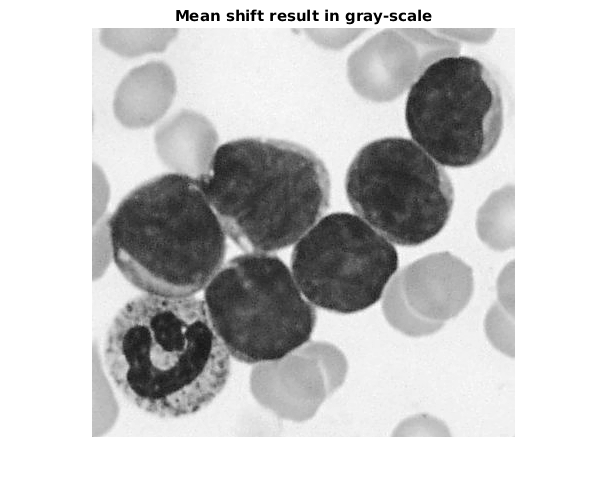
\includegraphics[scale=0.5]{img/final/meangran.png}
		\caption{Granulocite after Mean shift application}
		\label{fig:grangray}
\end{center}
\end{figure}
\begin{figure}
\begin{center}
		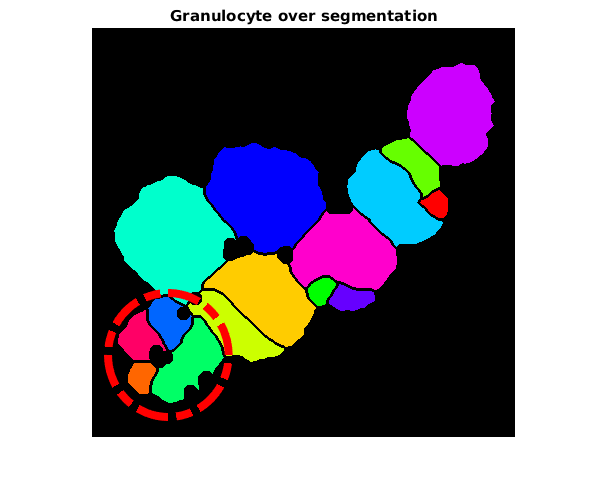
\includegraphics[scale=0.5]{img/final/fingran.png}
		\caption{Over-segmentation caused by the granulocyte}
		\label{fig:gran}
\end{center}
\end{figure}

The most important points that we focused in this thesis can be summarized in four sections:
\begin{enumerate}
\item preprocessing using the mean shift algorithm in order to delete all the differences of colour inside the cells;
\item extrapolation of the right and left component of the VFC force;
\item application of the skeleton in order to separate the overlapped cells;
\item recognize and count of the cells.
\end{enumerate}

\bigskip

Our method demonstrates that at this moment is better than everyone algorithm existing in literature. The only problem is the less robustness causing by the low quality images and the over-segmentation caused by the granulocytes. But as the literature says, this is the complex field in histologic image segmentation.

\bigskip

But is possible to resolve this robustness problem. As future works we want to implement a new kind of region linking in order to delete all the over-segmentation and a new points liking function to remove the skeleton side of the algorithm and use only the informations give by the VFC components. Another feature to implement is the region merging for the small areas in granulocyte cells, to overcome the over-segmentation of these last. 